

\chapter{Martingales}

\section{Definition and examples}
We are ready to start studying the processes known as
martingales, which generalize the ``balancing''
property exhibited by the fraction of white balls in
the Poly\'a urn experiment.

Let $(\Omega, \mathcal{F}, \mathrm{P})$ be a
probability space, equipped with an increasing family

\[
\mathcal{G}_1 \subset \mathcal{G}_2 \subset \mathcal{G}_3 \subset \ldots
\]

\noindent of sub-$\sigma$-algebras of $\mathcal{F}$. We refer
to such a family $(\mathcal{G}_n)_{n=1}^\infty$ as a
$\textbf{filtration}$. The $n$th $\sigma$-algebra
$\mathcal{G}_n$ represents the state of knowledge (of
an experimenter) about the probabilistic world
$(\Omega, \mathcal{F}, \mathrm{P})$ at time $n$. A
sequence of random variables $(X_n)_{n=1}^\infty$ is
said to be \textbf{adapted to the filtration
$(\mathcal{G}_n)_{n=1}^\infty$} if $X_n$ is
$\mathcal{G}_n$-measurable for any $n$; that is, if
the $n$th value in the sequence is known at time $n$.

\begin{defn}
Given a filtration $(\mathcal{G}_n)_{n=1}^\infty$, a
sequence $(X_n)_{n=1}^\infty$ of random variables is
called a \textbf{martingale} with respect to the filtration
if it satisfies:

\begin{enumerate}[label=\arabic*.]
\item $\mathbf{E}|X_n|<\infty$ for all $n\ge1$.

\item The sequence $(X_n)_{n=1}^\infty$ is adapted to the
filtration $(\mathcal{G}_n)_{n=1}^\infty$.

\item $\mathbf{E}\left(X_{n+1}\,|\,\mathcal{G}_n\right) =
X_n$
for all $n\ge 1$.
\end{enumerate}

\noindent If instead of property M3.\ the sequence satisfies
the condition
$\mathbf{E}\left(X_{n+1}\,|\,\mathcal{G}_n\right) \ge
X_n$,
it is called a \textbf{submartingale}. If it satisfies
$\mathbf{E}\left(X_{n+1}\,|\,\mathcal{G}_n\right) \le
X_n$,
it is called a \textbf{supermartingale}
\end{defn}

\begin{example}
(Simple random walk). Let $X_1, X_2, \ldots,$ be a
sequence of i.i.d. random variables with
$\mathrm{P}(X_n=1)=\tfrac12$,
$\mathrm{P}(X_n=-1)=\tfrac12$. Denote
$S_n = \sum_{k=1}^n X_n$. Define the filtration
$(\mathcal{G}_n)_n$ by
$\mathcal{G}_n = \sigma(X_1,\ldots,X_n)$ (the
$\sigma$-algebra generated by the first $n$ random
signs). Then the sequence $(S_n)_{n=1}^\infty$ (known
as ``simple symmetric random walk on $\Z$'') is a
martingale with respect to $(\mathcal{G}_n)_n$, since

\[
\mathbf{E}\left(S_n\,|\,\mathcal{G}_{n-1}\right) = \mathbf{E}\left(S_{n-1}+X_n\,|\,\mathcal{G}_{n-1}\right)
= S_{n-1} + \mathbf{E}\left(X_n\,|\,\mathcal{G}_{n-1}\right) = S_{n-1} + \mathbf{E}(X_n) = S_{n-1}.
\]

\end{example}

\begin{example}
(Random walk with balanced steps). More generally,
the cumulative sums $S_n=\sum_{k=1}^n S_n$ of an
i.i.d.\ sequence $X_1,X_2,\ldots$ where $X_n\sim F$
(the random walk with i.i.d. steps distributed
according to $F$) is a martingale with respect to the
filtration $\mathcal{G}_n=\sigma(X_1,\ldots,X_n)$ if
$\mathbf{E}(X_1)=0$. Even more generally, the r.v.'s
$X_1,X_2,\ldots$ can be assumed to be independent but
not identically distributed; if for any $n$ we have
that $\mathbf{E}|X_n|<\infty$ and
$\mathbf{E} X_n = 0$, then (by the same computation
as above) $S_n$ is a martingale.
\end{example}

\begin{example}
(Revealing information). Let $X$ be a random variable
and let $(\mathcal{G}_n)_{n=1}^\infty$ be a
filtration. The sequence $(X_n)_{n=1}^\infty$ defined
by $X_n = \mathbf{E}\left(X\,|\,\mathcal{G}_n\right)$
is a martingale. Intuitively, it is the sequence of
better and better estimates for the value of $X$ that
we can make as more and more information (represented
by the filtration) is revealed.
\end{example}

\noindent It is not difficult to check that if
$(X_n)_{n=1}^\infty$ is a martingale with respect to
a filtration $(\mathcal{G}_n)_{n=1}^\infty$ then
$(X_n)_{n=1}^\infty$ is also a martingale with
respect to its ``natural'' filtration
$\mathcal{H}_n=\sigma(X_1,\ldots,X_n) \subset
\mathcal{G}_n$.
This illustrates the fact that the filtration
$(\mathcal{G}_n)$ usually doesn't play a very major
role, but is simply a convenient way to represent the
information that is used to compute the sequence.

\begin{example}
(Discrete harmonic functions on a graph). Let
$G=(V,E)$ be a graph (assume $V$ is finite or
countable). A function $h:V\to\R$ is called
$\textbf{harmonic}$ if it satisfies the ``mean
value'' property

\[
h(x) = \frac{1}{\operatorname{deg}(x)}\sum_{y \sim x} h(y) \qquad (x\in V),
\]

\noindent where the notation $y\sim x$ means that $x,y$ are
neighbors and $\operatorname{deg}(x)$ is the number
of neighbors (the degree of $x$). Let
$X_0,X_1,X_2,\ldots$ be a \textbf{simple random walk on $G$};
that is, each $X_n$ is a $V$-valued random variable,
and the distribution of $X_{n+1}$ is defined
conditionally on $X_n$ by

\[
\mathrm{P}(X_{n+1} = y\,|\,X_n=x) = \begin{cases} \frac{1}{\operatorname{deg}(x)} & y\sim x, \\ 0 & y\nsim x.
\end{cases}
\]

\noindent The starting point $X_0$ of the walk can be a
deterministic vertex $x$ or a distribution on $V$.
Let $\mathcal{G}_n=\sigma(X_0,\ldots,X_n)$. Define a
sequence of real-valued random variables by
$M_n = h(X_n)$. As an exercise, we leave to the
reader to check that $(M_n)_{n=0}^\infty$ is a
martingale with respect to the filtration
$(\mathcal{G}_n)_{n=0}^\infty$
\end{example}

\begin{example}
(``Double or nothing''). Let $X_1,X_2,\ldots$ be an
i.i.d.\ sequence of random variables satisfying
$\mathrm{P}(X_n = 0) = \tfrac12, \mathrm{P}(X_n = 2)
= \tfrac12$.
Let $\mathcal{G}_n=\sigma(X_1,\ldots,X_n)$. Define
$M_n = \prod_{k=1}^n X_n$. Then

\[
\mathbf{E}\left(M_{n+1}\,|\,\mathcal{G}_{n}\right) = \mathbf{E}\left(M_{n} X_{n+1}\,|\,\mathcal{G}_n\right) = M_{n} \mathbf{E}\left(X_{n+1}\,|\,\mathcal{G}_n\right) = M_{n} \mathbf{E}{X_{n+1}} = M_n,
\]

\noindent so $(M_n)_{n=1}^\infty$ is a martingale with respect
to the filtration $(\mathcal{G}_n)_{n=1}^\infty$. The
meaning of the name ``double or nothing'' should be
obvious.
\end{example}

\begin{example}
(Multiplicative random walk). The previous example is
a special case of the following situation: let
$X_1, X_2, \ldots$ be an i.i.d. sequence of
nonnegative random variables with $\mathbf{E}(X_1)=1$.
Then by the same computation as above,
$M_n = \prod_{k=1}^n X_k$ is a martingale with
respect to the filtration
$\mathcal{G}_n = \sigma(X_1,\ldots,X_n)$.
\end{example}

\begin{example}
(Alexander Calder mobile sculptures). The mobile
sculptures pioneered by the American sculptor
Alexander Calder are a mechanical manifestation of a
martingale (Figure 1).

\begin{center}

\includegraphics[width=0.38\linewidth]{figures/caldermobile1.jpeg}\hspace{0.02\linewidth}%

\includegraphics[width=0.38\linewidth]{figures/caldermobile2.jpg}\\[0.6em]
{\small Figure 1: Some mobiles by Alexander Calder}
\end{center}

\noindent The idea is that the $n$th random variable
corresponds to the horizontal displacement of a
``node'' in the mobile as one descends the tree of
nodes starting from the upper support point of the
mobile. The fact that the tree is in static
equilibrium corresponds to the statement that the
center of mass of the subtree supported below each
node is at the same horizontal displacement as the
node itself, which can be thought of as a version of
the martingale equation
$\mathbf{E}\left(X_{n+1}\,|\,\mathcal{G}_n\right) =
X_n$.
\end{example}

\begin{example}
(Whippletrees). Another real-life example of the
martingale idea is in the mechanical device known as a
$\textbf{whippletree}$, used to divide force evenly
between several draught animals towing a load (Figure
2).

\begin{center}
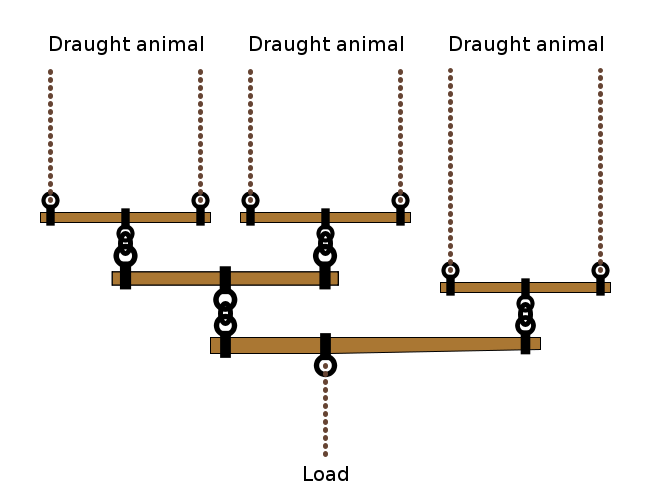
\includegraphics[width=0.45\linewidth]{figures/whippletree.png}\\[0.6em]
{\small Figure 2: An illustration of a whippletree (source:
Wikipedia)}
\end{center}

\end{example}

\begin{thm}

\begin{enumerate}[label=\arabic*.]
\item If $(X_n)_{n=1}^\infty$ is a martingale w.r.t.\ a
filtration $(\mathcal{G}_n)_{n=1}^\infty$, then for
$m< n$,
$\mathbf{E}\left(X_n\,|\,\mathcal{G}_m\right) = X_m$.

\item If $(X_n)_{n=1}^\infty$ is a supermartingale w.r.t.\
$(\mathcal{G}_n)_{n=1}^\infty$, then for $m< n$,
$\mathbf{E}\left(X_n\,|\,\mathcal{G}_m\right) \le
X_m$.

\item If $(X_n)_{n=1}^\infty$ is a submartingale w.r.t.\
$(\mathcal{G}_n)_{n=1}^\infty$, then for $m< n$,
$\mathbf{E}\left(X_n\,|\,\mathcal{G}_m\right) \ge
X_m$.
\end{enumerate}

\end{thm}

\begin{proof}
It is enough to prove claim 2., since 3.\ follows by
applying 2. to $-X_n$, and 1.~follows by combining
2.~and~3. Assume $X_n$ is a supermartingale, then
$X_m\ge
\mathbf{E}\left(X_{m+1}\,|\,\mathcal{G}_m\right)$
by the definition, and by induction on $k$,
$X_m\ge
\mathbf{E}\left(X_{m+k}\,|\,\mathcal{G}_m\right)$,
since if we showed this for $k-1$ then we have that

\begin{align*}
X_m &\ge \mathbf{E}\left(X_{m+1}\,|\,\mathcal{G}_m\right)
\ge \mathbf{E}\left(\mathbf{E}\left(X_{m+1+(k-1)}\,|\,\mathcal{G}_{m+1}\right)\,|\,\mathcal{G}_m\right)
= \mathbf{E}\left(X_{m+k}\,|\,\mathcal{G}_m\right).
\end{align*}

\end{proof}

\begin{thm}

\begin{enumerate}[label=\arabic*.]
\item If $(X_n)_n$ is a martingale w.r.t.\
$(\mathcal{G}_n)_n$ and $\varphi:\R\to\R$ is a convex
function such that $\mathbf{E}|\varphi(X_n)|<\infty$
for all $n$, then $(\varphi(X_n))_n$ is a
submartingale.

\item If $(X_n)_n$ is a submartingale w.r.t.\
$(\mathcal{G}_n)_n$ and $\varphi:\R\to\R$ is a weakly
increasing convex function such that
$\mathbf{E}|\varphi(X_n)|<\infty$ for all $n$, then
$(\varphi(X_n))_n$ is a submartingale.
\end{enumerate}

\end{thm}

\begin{proof}
By Jensen's inequality,
$\mathbf{E}\left(\varphi(X_{n+1})\,|\,\mathcal{G}_n\right)
\ge
\varphi\left(\mathbf{E}\left(X_{n+1}\,|\,\mathcal{G}_n\right)\right)$,
and this is $= \varphi(X_n)$ in the case of the first
claim, or $\ge \varphi(X_n)$ in the case of the
second.
\end{proof}

\begin{cor}
Let $p\ge 1$. If $(X_n)_n$ is a martingale w.r.t.\
$(\mathcal{G}_n)_n$ and $\mathbf{E}|X_n|^p<\infty$
for all $n$, then $|X_n|^p$ is a submartingale
w.r.t.\ $(\mathcal{G}_n)_n$.
\end{cor}

\begin{cor}
\label{cor-positive-part}

\begin{enumerate}[label=\arabic*.]
\item If $(X_n)_{n=1}^\infty$ is a submartingale then
$\big((X_n-a)_+\big)_{n=1}^\infty$ is a submartingale
(where for a real number $x$, $x_+ = \max(x,0)$ is
the positive part of $x$).

\item If $(X_n)_{n=1}^\infty$ is a supermartingale then for
any $a\in\R$, $(X_n\wedge a)_{n=1}^\infty$ is a
supermartingale.
\end{enumerate}

\end{cor}

\section{The martingale transform and investment strategies}
Let $(\mathcal{G}_n)_{n=0}^\infty$ be a filtration.
Assume that we are given a sequence
$(X_n)_{n=0}^\infty$ that is adapted to the
filtration. Each increment $X_n-X_{n-1}$ can be
thought of as representing an investment opportunity
at time $n$. For example, $X_n$ can represent the
price of a stock or other financial asset (which in
the lingo of finance is referred to, somewhat
ironically, as a ``security'') on day $n$, so that
$X_n-X_{n-1}$ will be the gain or loss of an investor
holding one unit of the asset during day $n$. The
$\textbf{martingale transform}$$H\bullet X$ is a new
sequence of random variables representing the
accumulated profits of an investor employing a
predefined investment strategy, represented by a
sequence
$(H_n)_{n=1}^\infty$.\footnote{The name ``martingale transform'' is a poor choice,
as it seems to imply that $H\bullet X$ is defined
only when $(X_n)_n$ is a martingale. This is not the
case, although it's true that the most interesting
cases are when $(X_n)_n$ is a submartingale or
supermartingale or both.}

To make this more precise, we say that a sequence
$(H_n)_{n=1}^\infty$ is $\textbf{predictable}$ with
respect to the filtration
$(\mathcal{G}_n)_{n=0}^\infty$ if for any $n\ge 1$,
$H_n$ is $\mathcal{G}_{n-1}$-measurable. Think of
$H_n$ as representing the number of investment units
the investor holds during the $n$th trading day. An
investment strategy must have this property, since
(unless the investor is equipped with a crystal ball)
the decision of how much to invest at time $n$ must
depend only on information available at time $n-1$.
Given a $(\mathcal{G}_n)_n$-adapted sequence
$(X_n)_{n=0}^\infty$ and a predictable sequence
$(H_n)_{n=1}^\infty$, we define the sequence
$H\bullet X$ by

\[
(H\bullet X)_n = \sum_{m=1}^n H_m(X_m-X_{m-1}).
\]

\begin{thm}
\label{thm-marting-transform}

\begin{enumerate}[label=\arabic*.]
\item If $(X_n)_{n=0}^\infty$ is a supermartingale and
$(H_n)_{n=1}^\infty$ is predictable, and for any $n$,
$H_n$ is bounded and nonnegative, then $H\bullet X$
is a supermartingale.

\item If $(X_n)_{n=0}^\infty$ is a submartingale and
$(H_n)_{n=1}^\infty$ is predictable, and for any $n$,
$H_n$ is bounded and nonnegative, then $H\bullet X$
is a submartingale.

\item If $(X_n)_{n=0}^\infty$ is a martingale and
$(H_n)_{n=1}^\infty$ is predictable, and for any $n$,
$H_n$ is bounded, then $H\bullet X$ is a martingale.
\end{enumerate}

\end{thm}

\begin{proof}
We prove the first claim (the other ones are
similar). It is obvious that $(H\bullet X)_n$ is
adapted to $(\mathcal{G}_n)_n$, and furthermore, by
the assumptions that $H_n$ is bounded and
nonnegative, and the usual properties of conditional
expectation, we get that

\begin{align*}
\mathbf{E}\left((H\bullet X)_{n+1}\,|\,\mathcal{G}_n\right) &=
\mathbf{E}\left((H\bullet X)_{n}\,|\,\mathcal{G}_n\right) +
\mathbf{E}\left(H_{n+1}(X_{n+1}-X_n)\,|\,\mathcal{G}_n\right) \\
&= (H\bullet X)_n +
H_{n+1} \mathbf{E}\left(X_{n+1}-X_n\,|\,\mathcal{G}_n\right) \le (H\bullet X)_n.
\end{align*}

\end{proof}

\noindent A random variable $N$ taking values in
$\{1,2,\ldots\}\cup \{\infty\}$ is said to be a
$\textbf{stopping time}$ with respect to the
filtration $(\mathcal{G}_n)_{n=0}^\infty$ if for any
$n\ge0$, the event $\{ N=n \}$ is in $\mathcal{G}_n$.
That means that the decision to stop at time $n$
depends only on information available at that time.
Given a stopping time $N$, one possible investment
strategy (a version of the classic ``buy and hold'')
is to buy one investment unit at time $0$ and hold it
until time $N$. In other words, we may define a
sequence $(H_n)_n$ by

\[
H_n = \mathbf{1}_{\{n\le N\}}, \qquad n\ge 1.
\]

\noindent Note that
$\{ n\le N\} = \{N\le n-1\}^\textrm{c} \in
\mathcal{G}_{n-1}$,
so $(H_n)_n$ is a predictable sequence, and we have

\[
(H\bullet X)_n = X_{N\wedge n} - X_0.
\]

\begin{thm}
\label{thm-stopping-mart}
If $N$ is a stopping time and $(X_n)_{n=0}^\infty$ is
a supermartingale (respectively, submartingale,
martingale), then $(X_{n\wedge N})_{n=0}^\infty$ is a
supermartingale (respectively, submartingale,
martingale).
\end{thm}

\begin{proof}
By Theorem \ref{thm-marting-transform},
$X_{N\wedge n} - X_0$ is a supermartingale. Adding
the constant sequence $Y_n=X_0$ to it (which is a
martingale) gives a supermartingale.
\end{proof}

\section{The upcrossing inequality}
An essential step on the way to the martingale
convergence theorem is an inequality bounding the
expected number of times a submartingale may cross
between two values $a<b$. Let $(X_n)_{n\ge 0}$ be a
submartingale, and fix $a<b$. We define an increasing
sequence of stopping times

\[
N_0 < N_1 < N_2 < \ldots
\]

\noindent recursively by setting $N_0=-1$, and

\begin{align*}
N_{2k-1} &= \inf \{ m > N_{2k-2}\,:\,X_m\le a\}, \\
N_{2k} &= \inf \{ m > N_{2k-1}\,:\,X_m\ge b\},
\end{align*}

\noindent for each $k\ge 1$. It is easy to check that the
sequence

\[
H_m = \begin{cases} 1 &\textrm{ if }N_{2k-1}<m\le N_{2k}\textrm{ for some }k, \\
0 & \textrm{otherwise},
\end{cases}
\]

\noindent is a predictable sequence; it corresponds to the
strategy of buying an investment unit as soon as the
price dips below $a$ and selling the next time it
goes above $b$. Let

\[
U_n = U_n(a,b) = \sup \{ k\ge 0\,:\,N_{2k}\le n\}.
\]

\noindent We refer to $U_n$ as the number of
$\textbf{upcrossings}$ the sequence $(X_n)_n$
completed up to time $n$ (where an upcrossing
represents a cycle of going from a value below $a$ to
a value above $b$).

\begin{thm}
We have

\[
\mathbf{E} U_n \le \frac{1}{b-a}\left( \mathbf{E}(X_n-a)_+ - \mathbf{E}(X_0-a)_+ \right).
\]

\end{thm}

\begin{proof}
Define $Y_m = a+(X_m-a)_+$. By Corollary
\ref{cor-positive-part}, $(Y_m)_m$ is a submartingale.
Note that $Y_m\le a$ if and only if $X_m\le a$ and
$Y_m\ge b$ if and only if $X_m\ge b$, so the
upcrossing number associated with the sequence
$(Y_m)_m$ is $U_n$, the same as for $(X_m)_m$.
Furthermore, we have the inequality

\[
(b-a)U_n \le (H\bullet Y)_n,
\]

\noindent since $(H\bullet Y)$ would represent the profit made
on using the investment strategy $H$ to invest in the
sequence $Y_m$; each of the $U_n$ upcrossings gives a
profit of $b-a$, and there is possibly a last
incomplete stretch of investment when $Y_m$ dips to
$a$ (unlike $X_m$, $Y_m$ never goes strictly below
$a$) but has not yet increased above $b$, which gives
additional nonnegative profit. Finally, by Theorem
\ref{thm-marting-transform},
$\mathbf{E}((1-H)\bullet Y)_n\ge 0$, so we have

\begin{align*}
\mathbf{E}(H\bullet Y)_n &\le \mathbf{E}(H\bullet Y)_n + \mathbf{E}((1-H)\bullet Y)_n = \mathbf{E}(1\bullet Y)_n \\ &= \mathbf{E}(Y_n-Y_0) = \mathbf{E}(X_n-a)_+ - \mathbf{E}(X_0-a)_+.
\end{align*}

\noindent Combining the two inequalities gives the result.
\end{proof}

\section{The martingale convergence theorem}
With the help of the upcrossing inequality we can
prove:

\begin{thm}[The martingale convergence theorem]
If $(X_n)_{n=0}^\infty$ is a submartingale with
$\sup_{n\ge 0}\mathbf{E} (X_n)_+ < \infty$, then the
limit

\[
X = \lim_{n\to\infty} X_n
\]

\noindent exists almost surely and satisfies
$\mathbf{E}|X|<\infty$.
\end{thm}

\begin{proof}
For each $a<b$, let

\[
U(a,b) = \sup_{n\ge0} U_n(a,b)
\]

\noindent denote the total number of $(a,b)$-upcrossings over
the entire history of the sequence (which may be
infinite). Since

\[
\mathbf{E} U_n(a,b) \le \frac{1}{b-a} \mathbf{E}(X_n-a)_+ \le \frac{1}{b-a} \left[ a + \mathbf{E} (X_n)_+ \right],
\]

\noindent by the assumption on $\sup_n \mathbf{E}(X_n)_+$ and
the monotone convergence theorem we also get that
$\mathbf{E} U(a,b) < \infty$, hence $U(a,b)<\infty$
almost surely. It follows that the event

\[
A = \bigcup_{\stackrel{a<b}{a,b\in\mathbb{Q}}} \{ U(a,b) = \infty \}
\]

\noindent has probability $0$. On the almost sure complementary
event $A^c$, the only way the sequence $X_n$ can
diverge is by converging to $\pm \infty$. In other
words, the limit

\[
X = \lim_{n\to\infty} X_n
\]

\noindent exists as a generalized r.v.\ taking values in
$\R\cup\{\pm\infty\}$. But then by Fatou's lemma we
have that

\[
\mathbf{E} X_+ \le \liminf_{n\to\infty} \mathbf{E} (X_n)_+ \le \sup_{n\ge 0} \mathbf{E}(X_n)_+ < \infty,
\]

\noindent which also implies that $X<\infty$ a.s. Similarly,
note that

\[
\mathbf{E} (X_n)_- = \mathbf{E} (X_n)_+ - \mathbf{E}(X_n) \le \mathbf{E} (X_n)_+ - \mathbf{E} X_0,
\]

\noindent since $X_n$ is a submartingale, so again by Fatou's
lemma we have

\[
\mathbf{E} X_- \le \liminf_{n\to\infty} \mathbf{E} (X_n)_- \le \sup_n \mathbf{E}(X_n)_+ - \mathbf{E} X_0 < \infty,
\]

\noindent which shows that $X>-\infty$ a.s. We have shown that
$X_n$ converges a.s. to a finite limit both of whose
positive and negative parts are integrable, so the
proof is complete.
\end{proof}

\begin{cor}
\label{mart-conv-cor}

\begin{enumerate}[label=\arabic*.]
\item If $(X_n)_n$ is a submartingale bounded from above,
i.e., there is an $M\in\R$ such that $X_n\le M$ for
all $n$, then $X_n\to X$ a.s.\ where the limiting
r.v.\ satisfies $\mathbf{E} X \ge \mathbf{E} X_0$.

\item If $(X_n)_n$ is a supermartingale bounded from below,
i.e., there is an $M$ such that $X_n\ge M$ for all
$n$, then $X_n\to X$ a.s.\ where the limiting r.v.\
satisfies $\mathbf{E} X \le \mathbf{E} X_0$.
\end{enumerate}

\end{cor}

\section{$L_p$ spaces and modes of convergence}
In this section we summarize some facts about the
$L_p$ spaces (which are function spaces that play a
central role in many parts of mathematical analysis
and in particular in probability theory) and the
different modes of convergence for random variables.
Previously we discussed the notions of
$\textbf{convergence in probability}$,
$\textbf{almost sure convergence}$ and
$\textbf{convergence in distribution}$. Other useful
senses in which random variables may be said to
converge to a limit are $\textbf{uniform convergence}$
(equivalent to \textbf{convergence in the space $L_\infty$})
and \textbf{convergence in the $L_p$ space}.

\begin{defn}
Let $(\Omega, \mathcal{F}, \mathrm{P})$ be a
probability space. For $1\le p<\infty$, we associate
with our probability space a function space
$L_p(\Omega, \mathcal{F}, \mathrm{P})$ (often denoted
as $L_p(\Omega)$ or simply $L_p$ when the context is
clear), defined by

\[
L_p(\Omega, \mathcal{F}, \mathrm{P}) = \{ X:\Omega\to\mathbb{C}\textrm{ is a random variable}\,:\, \mathbf{E}|X|^p < \infty \}.
\]

\noindent Elements of $L_p$ are considered only up to almost
sure equivalence\footnote{That is, formally, the elements of $L_p$ are not
random variables but equivalence classes of random
variables modulo almost sure equivalence, but in
practice no one bothers to say things in this formal
language.}. The $p$-norm of a
random variable $X\in L_p$ is defined by

\[
\lVert X\rVert_p = \left( \mathbf{E} |X|^p\right)^{1/p}.
\]

\noindent For $p=\infty$ one may also define the space
$L_\infty$ with an associated $\infty$-norm
$\lVert\cdot\rVert_\infty$ by

\[
L_\infty(\Omega,\mathcal{F},\mathrm{P}) = \{ X:\Omega\to\mathbb{C}\textrm{ is a random variable}\,: X\textrm{ is essentially bounded} \},
\]

\noindent where \textbf{essentially bounded} means that after
modifying $X$ on a set of $\mathrm{P}$-measure $0$
one gets a bounded function. The $\infty$-norm
$\lVert X\rVert_\infty$ is defined as the infimum of
all numbers $M$ which are essential bounds of $X$
(i.e., all $M$ such that $\mathrm{P}(|X|\le M)=1$).
\end{defn}

\noindent The space $L_p$ equipped with the norm
$\lVert \cdot \rVert_p$ becomes a metric space. A
fundamental fact from analysis is:

\begin{thm}
For $1\le p\le \infty$, $L_p$ is a complete metric
space. That is, every Cauchy sequence in $L_p$ is
convergent.
\end{thm}

\noindent Since $L_p$ is actually a normed space, the theorem
above means it is a Banach space (a complete normed
vector space). For $p=2$ it is also a Hilbert space
(a complete inner product space), since it may be
equipped with the inner product

\[
\langle X,Y\rangle = \mathbf{E}(X\overline{Y}).
\]

\noindent The elements of $L_2$ are referred to as
$\textbf{square-integrable random variables}$
(equivalently, random variables with finite variance).
Note that the Cauchy-Schwartz inequality guarantees
that $\langle X,Y\rangle$ is defined and finite when
$X,Y\in L_2$.

\begin{defn}
The modes of convergence of a sequence of random
variables $(X_n)_{n=1}^\infty$ to a limiting random
variable $X$ are defined as follows:

\begin{enumerate}[label=\arabic*.]
\item \textbf{Convergence in probability:}$X_n \to X$ in
probability if for any $\epsilon>0$, we have
$\lim_{n\to\infty} \mathrm{P}(|X_n-X|>\epsilon)\to 0$
as $n\to\infty$.

\item \textbf{Almost sure convergence:}$X_n\to X$ almost surely
if
$\mathrm{P}(X_n\to X\ \textrm{ as }n\to\infty) = 1$.

\item \textbf{Convergence in $L_p$, $1\le p<\infty$:}$X_n\to X$
in $L_p$ if $\mathbf{E}|X_n-X|^p \to 0$ as
$n\to\infty$. For $p=1$ this is also called
\textbf{convergence in the mean}.

\item \textbf{Convergence in $L_\infty$:}$X_n\to X$ in $L_\infty$
in $L_\infty$ if $\lVert X_n-X\rVert_\infty\to 0$ as
$n\to\infty$.

\item \textbf{Convergence in distribution:}$X_n\to X$ in
distribution if $\mathbf{E} g(X_n)\to \mathbf{E} g(X)$
for any bounded continuous function $g:\R\to\R$.
\end{enumerate}

\end{defn}

\noindent It should be noted that the concept of convergence in
distribution is qualitatively different from the other
modes of convergence, in that it does not require the
random variables $X, X_1, X_2, \ldots$ to be defined
on the same probability space. The convergence in this
case is of the \emph{probabilities} and other statistical
measures of the distributions of the random variables
(i.e., expectations of functions applied to $X_n$,
moments, characteristic functions, etc.), not of the
values of the random variables themselves in some
experiment in which they are sampled.

The proof of the following theorem is left to the
reader as an exercise in scholarly research (meaning,
for each of the claims either try to prove it by
yourself, or track down the proofs in a textbook ---
you will probably learn other useful things while
searching!)

\begin{thm}
The following relationships exist between the
different modes of convergence:

\begin{enumerate}[label=\arabic*.]
\item If $X_n\to X$ almost surely then $X_n\to X$ in
probability. The converse is not true.

\item If $X_n\to X$ in probability then $X_n \to X$ in
distribution. The converse is not true, even in the
case when $(X_n)_{n=1}^\infty$ and $X$ are all
defined on the same probability space.

\item If $X_n\to X$ in distribution then there exists a
sequence $(Y_n)_{n=1}^\infty$ and a random variable
$Y$, all defined on the same probability space, such
that $Y_n \stackrel{\textrm{D}}{=} X_n$ for all $n$,
$Y\stackrel{\textrm{D}}{=} X$, and $Y_n\to Y$ almost
surely.

\item If $X_n\to X$ almost surely and the convergence is
dominated (in the sense of the dominated convergence
theorem), then $X_n\to X$ in $L_1$.

\item If $X_n\to X$ in probability then there exists a
subsequence $(X_{n_k})_{k=1}^\infty$ such that
$X_{n_k}\to X$ almost surely.

\item If $X_n\to X$ in $L_p$ for some $1\le p \le\infty$
then there exists a subsequence
$(X_{n_k})_{k=1}^\infty$ such that $X_{n_k}\to X$
almost surely.

\item If $X_n\to X$ in $L_p$ for some $1\le p\le\infty$
then $X_n\to X$ in $L_q$ for any $1\le q\le p$.

\item If $X_n \to X$ in $L_\infty$ then $X_n\to X$ almost
surely.

\item If $X_n\to X$ in probability, then $X_n\to X$ in $L_1$
if and only if $(X_n)_{n=1}^\infty$ is uniformly
integrable (see the next section for the definition of
uniform integrability).
\end{enumerate}

\end{thm}

\section{Martingale convergence in $L_p$}
In certain applications a martingale may not be
bounded but can still be shown to converge based on
boundedness in $L_p$ and similar conditions. The
following results give such conditions. Proofs can be
found in [Dur2010], sections 5.4--5.5.

\begin{thm}[Martingale convergence theorem in $L_p$, $p>1$]
Let $1<p\le \infty$. If $(X_n)_{n=1}^\infty$ is a
martingale and $\sup_n \mathbf{E} |X_n|^p<\infty$,
then $X_n$ converges to a limit $X$ almost surely and
in $L_p$.
\end{thm}

\noindent Note that the above theorem is only valid for $p>1$.
For $p=1$ it is not enough to require that the
martingale be bounded in $L_1$. A stronger condition
is needed, that of uniform integrability. A family of
random variables $(X_i)_{i\in I}$ is called
$\textbf{uniformly integrable}$ if for any
$\epsilon>0$ there exists an $M>0$ such that

\[
\mathbf{E}( |X_i| \mathbf{1}_{\{|X_i|>M\}} ) < \epsilon \ \ \ \textrm{for all }i\in I.
\]

\noindent It is easy to see that a uniformly integrable family
is bounded in $L_1$. Some examples of uniformly
integrable families are:

\begin{enumerate}[label=\arabic*.]
\item A family of random variables that are all dominated
by a single integrable r.v.\ $Y$, i.e., $|X_i|\le Y$
for all $i\in I$. (Obvious.)

\item The family of conditional expectations
$\mathbf{E}\left(X\,|\,\mathcal{G}\right)$ where $X$
is an integrable r.v.\ and $\mathcal{G}$ ranges over
all sub-$\sigma$-fields of $\mathcal{F}$. (See
Theorem 5.5.1 in [Dur2010].)

\item Let $1< p\le \infty$. Any bounded family of random
variables in $L_p$ (i.e., a family $(X_i)_{i\in I}$
such that for some constant $C>0$,
$\lVert X_i \rVert_p\le C$ for all $i\in I$) is
uniformly integrable.

\begin{xexercise}
Prove this statement, and give a counterexample that
explains why the claim is not true for $p=1$.
\end{xexercise}
\end{enumerate}

\begin{thm}[Martingale convergence theorem in $L_1$]
Let $(X_n)_{n=1}^\infty$ be a submartingale. The
following conditions are equivalent:

\begin{enumerate}[label=\arabic*.]
\item $(X_n)_{n=1}^\infty$ is uniformly integrable.

\item $(X_n)_{n=1}^\infty$ converges a.s.\ and in $L_1$.

\item $(X_n)_{n=1}^\infty$ converges in $L_1$.
\end{enumerate}

\noindent If $(X_n)_{n=1}^\infty$ is a martingale and not just
a submartingale, then the above conditions are also
equivalent to the existence of an integrable random
variable $X$ such that
$X_n = \mathbf{E}\left(X\,|\,\mathcal{G}_n\right)$
for all $n$ (i.e., the martingale is an instance of
the ``revealing information'' family of examples).
\end{thm}

\begin{xexercise}
Prove directly from the definitions that if
$(X_n)_{n=1}^\infty$ is a martingale with respect to
a filtration $(\mathcal{G}_n)_{n=1}^\infty$ and
$X_n\to X$ in $L_1$, then
$X_n = \mathbf{E}\left(X\,|\,\mathcal{G}_n\right)$.
\end{xexercise}

\noindent As a corollary we get:

\begin{thm}[Lévy's martingale convergence theorem]
\label{eq:levy-martingale-conv}
If $(\mathcal{G}_n)_{n=1}^\infty$ is an increasing
family of sub-$\sigma$-algebras of $\mathcal{F}$, and
$X\in L_1(\Omega)$ is a random variable, then

\[
\mathbf{E}\left(X\,|\,\mathcal{G}_n\right) \to \mathbf{E}\left(X\,|\,\mathcal{G}_\infty\right) \textrm{ a.s. as }n\to\infty,
\]

\noindent where
$\mathcal{G}_\infty = \vee_{n=1}^\infty \mathcal{G}_n
= \sigma\left(\cup_{n=1}^\infty \mathcal{G}_n\right)$
is the $\sigma$-algebra generated by the
$\mathcal{G}_n$'s. Similarly, for any event
$A\in \mathcal{F}$ we have

\[
\mathrm{P}\left(A\,|\,\mathcal{G}_n\right) \to \mathrm{P}\left(A\,|\,\mathcal{G}_\infty\right) \textrm{ a.s. as }n\to\infty
\]

\noindent In particular, if $A \in \mathcal{G}_\infty$ then we
have

\begin{equation*} \tag{8}\label{eq:levy-zero-one}
\mathrm{P}\left(A\,|\,\mathcal{G}_n\right) \to \mathbf{1}_A \textrm{ a.s. as }n\to\infty.
\end{equation*}

\noindent (This last fact is sometimes called
$\textbf{Lévy's 0-1 law}$.)
\end{thm}

\begin{xexercise}
Use (\ref{eq:levy-zero-one}) to give a new proof of
Kolmogorov's 0-1 law, which we learned about in the
previous quarter.
\end{xexercise}

